\section{Interface Utilisateur}

\begin{frame}{Interface Utilisateur}
\setlength{\parindent}{5ex}
Implémentation de différentes langues au sein du jeu :

\begin{figure}
    \centering
    
\includegraphics[width=12cm]{img/ui/mainmenu/fr.png}
    \caption{Français}
    \label{fig:fr}
\end{figure}
\begin{figure}
    \centering
    
\includegraphics[width=12cm]{img/ui/mainmenu/en.png}
    \caption{Anglais}
    \label{fig:en}
\end{figure}
\begin{figure}
    \centering
    
\includegraphics[width=12cm]{img/ui/mainmenu/es.png}
    \caption{Espagnol}
    \label{fig:es}
\end{figure}

\end{frame}


\begin{frame}{Interface Utilisateur - Suite}

\begin{figure}
    \centering
    
\includegraphics[width=6cm]{img/ui/selector.png}
    \caption{Sélection de la langue sous l'onglet Paramètres}
    \label{fig:uilangset}
\end{figure}

\begin{figure}
    \centering
    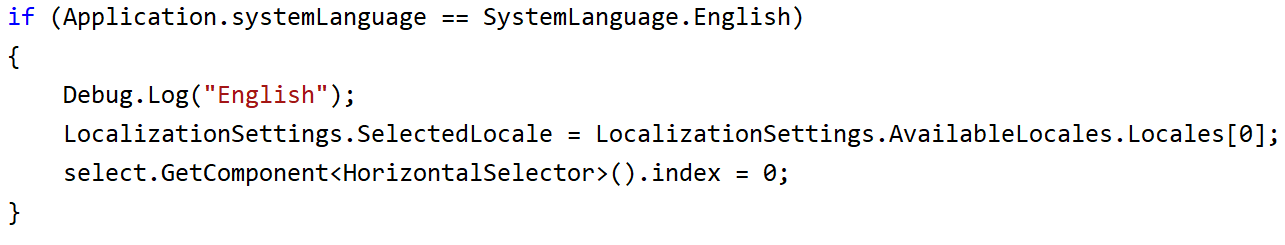
\includegraphics[width=12cm]{img/ui/mainmenu/code.png}
    \caption{Script gérant les langues, ici pour l'anglais}
    \label{fig:uilang}
\end{figure}

\end{frame}

\begin{frame}{Interface Utilisateur - Suite}

\begin{figure}
    \centering
    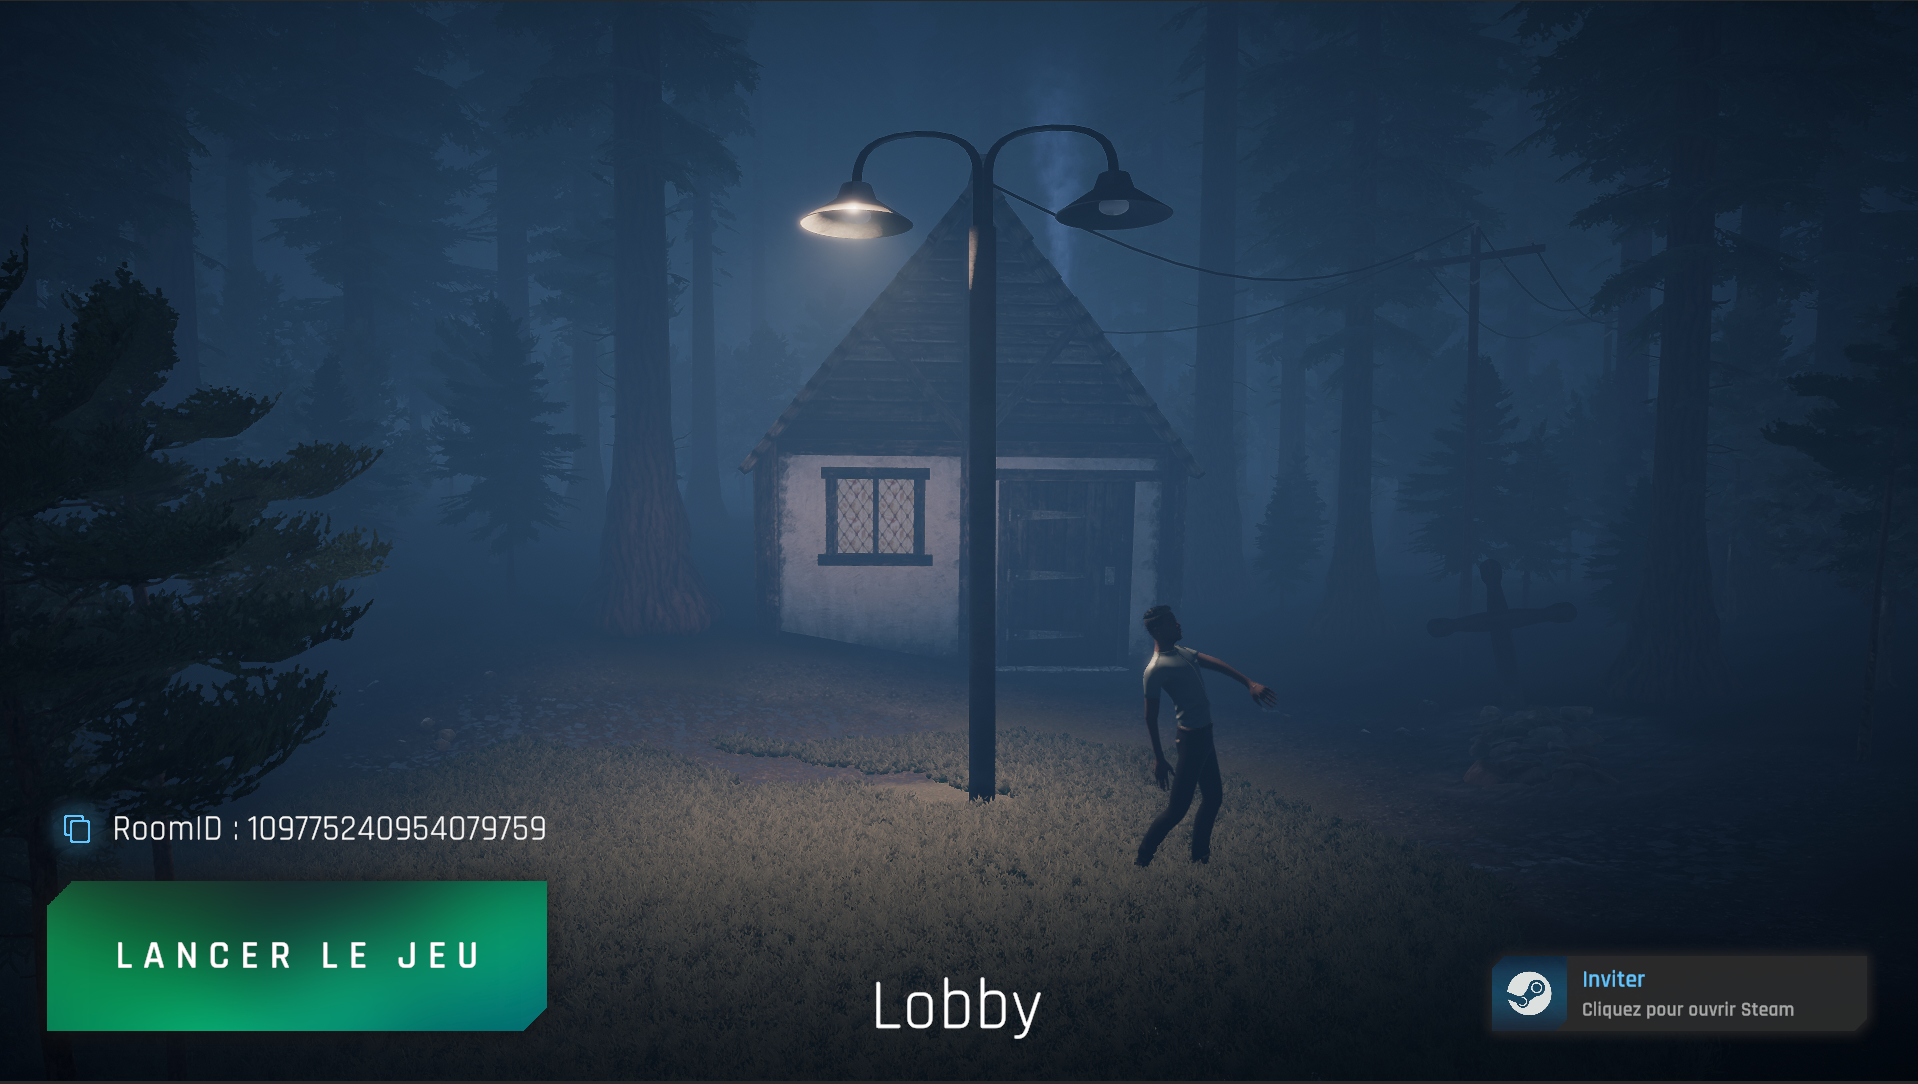
\includegraphics[width=10cm]{img/ui/lobby.png}
    \caption{Hall de jeu}
    \label{fig:lobby}
\end{figure}

\end{frame}